% !TEX encoding = UTF-8
% !TEX TS-program = pdflatex
% !TEX root = ../tesi.tex
% !TEX spellcheck = it-IT

%**************************************************************
\chapter{L'azienda}
\label{cap:azienda}
%**************************************************************
\intro{Questo capitolo tratta dettagliatamente della azienda ospitante, il suo \emph{business}, l'organizzazione interna e l'innovazione.}\\




%***************************************************************************************
\section{Presentazione azienda}
Questa sezione descrive l'azienda che ha ospitato lo \emph{stage}, elencando generalità e la struttura generale dell'azienda. Inoltre si illustrano alcuni prodotti e i servizi offerti da Nextep srl, alla propria clientela.

\subsection{L'azienda}
L'azienda con cui ho svolto lo stage formativo è Nextep srl\footnote{\url{http://www.nextep.it/}}, la cui sede operativa si trova a Carmignano Di Brenta(PD). Nextep è una società fondata nel 2000 che opera nel settore dell'informatica e della comunicazione. Il \emph{\gls{core business}} dell'azienda, è riconosciuto nelle attività di progettazione, realizzazione e gestione di infrastrutture di \emph{Information and Digital Communication Technology}. L'organico di Nextep srl è formato da una ventina di persone, suddivise tra \emph{web marketing} e tecnici (sviluppatori, grafici e sistemisti). L'ambiente di lavoro è condiviso con altre due aziende: Allos  e Zero12. Allos si occupa della formazione del capitale umano di organizzazioni medio grandi, mentre Zero12  si occupa di servizi \emph{cloud} e applicazioni \emph{mobile}. Il risultato è un ambiente di \emph{co-working}, dove le competenze del singolo vengono messe a disposizione di tutti, in modo da facilitare la crescita professionale dei dipendenti delle varie aziende. Non è raro che le tre aziende collaborino tra di loro per la realizzazione di alcuni progetti.
\begin{figure}[h]
\centering

\includegraphics[scale=0.20]{immagini/logo_nextep}
\caption{Logo di Nextep srl}
\label{fig:logo_nextep}
\end{figure}

\subsection{Prodotti e servizi}
Il principale settore di attività dell'azienda è il \emph{Web}. Nextep è specialista nella progettazione e sviluppo di siti \emph{web}, portali, \emph{social intranet} e soluzioni di \emph{e-commerce}. L'azienda fornisce sistemi per il \emph{knowledge management}, che sono dei sistemi per raccogliere, sviluppare, conservare e rendere accessibile la conoscenza delle persone che fanno parte di una organizzazione. Si occupa inoltre dello sviluppo di  applicazioni mobile. L'azienda pone il suo focus, nella realizzazione di sistemi con interfacce innovative e soprattutto accessibili all'utente, grazie alle competenze acquisite nel ramo della \emph{User Interface} e \emph{User Experience}. Realizza sistemi per l'integrazione con tecnologie e servizi di \emph{Cloud Computing}.\\
%Nello specifico l'azienda si occupa di:
%\begin{itemize}
%\item Progettazione e sviluppo di siti web e portali;
%\item Progettazione e sviluppo di Social Intranet e capitalizzazione della cultura aziendale;
%\item Progettazione e sviluppo di soluzioni di e-commerce;
%\item Studio, Progettazione e Realizzazione di Applicazioni Mobile;
%\item Studio e Progettazione delle Grafica/User Experience (UX);
%\item Integrazione con tecnologie e servizi di Cloud Computing;
%\item Analisi e progettazione di ecosistemi per siti web, portali, social internet, infrastrutture IT.
%\item Analisi, Ideazione e Realizzazione di azioni di web marketing.
%\end{itemize}
I principali servizi offerti da Nextep srl ai propri clienti sono:
\begin{itemize}
\item Fornitura di servizi a canone (\emph{server virtuali}, applicazioni \emph{web}, servizi di \emph{monitoring} di infrastrutture \emph{\gls{ict}}, \emph{backup-online}, canoni di assistenza e manutenzione dei sistemi, canoni di gestione dei sistemi);
\item Elaborazione dati, analisi e supporto decisionale in ambito \emph{web marketing}, \emph{social marketing} e \emph{social intranet};
%\item Consulenza e formazione di web marketing, social marketing, web analytics;
\item Servizio Clienti, attività di supporto tecnico e di gestione di infrastrutture \emph{\gls{ict}} e siti \emph{web}.
\end{itemize}
\begin{figure}[h]
\centering
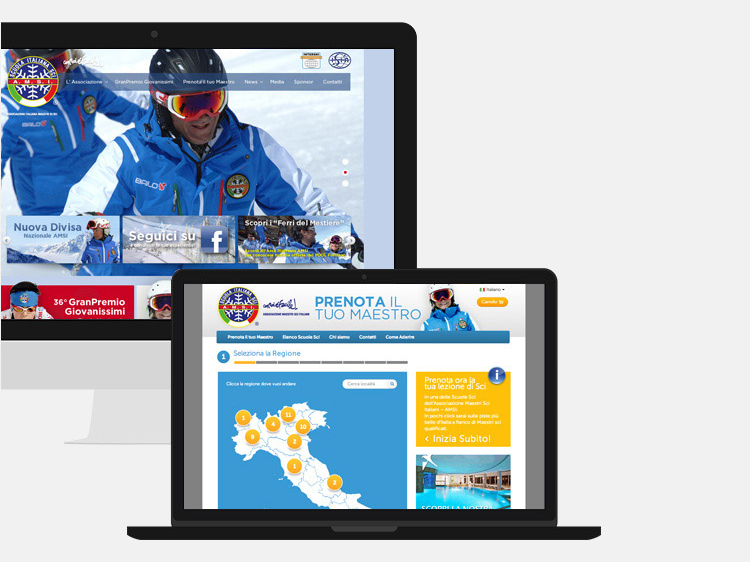
\includegraphics[scale=0.35]{immagini/amsi.jpg}
\caption{Sito Associazione Maestri Sci Italiani: realizzato da Nextep. Immagine tratta da \href{http://www.nextep.it/}{Nextep}}
\label{fig:amsi}
\end{figure}
In particolare l'azienda, fornisce servizi per migliorare l'efficacia delle strategie di comunicazione \emph{web}, dedicando particolare attenzione alla reputazione e all'identità digitale. Collabora, inoltre, assieme alle aziende nella gestione delle informazioni digitali, della sicurezza e della disponibilità dei dati e delle applicazioni. Infine nel ramo del \emph{marketing}, Nextep fornisce consulenza \emph{web marketing}, \emph{social marketing} e \emph{web analytics}.

\subsection{Tecnologie di riferimento}
Essendo il \emph{web} un settore soggetto a continue evoluzioni, le tecnologie utilizzate cambiano col tempo. Nextep cerca di aggiornare le tecnologie utilizzate, in modo da fornire ai propri clienti prodotti sempre migliori e innovativi.
\begin{figure}[h]
\centering
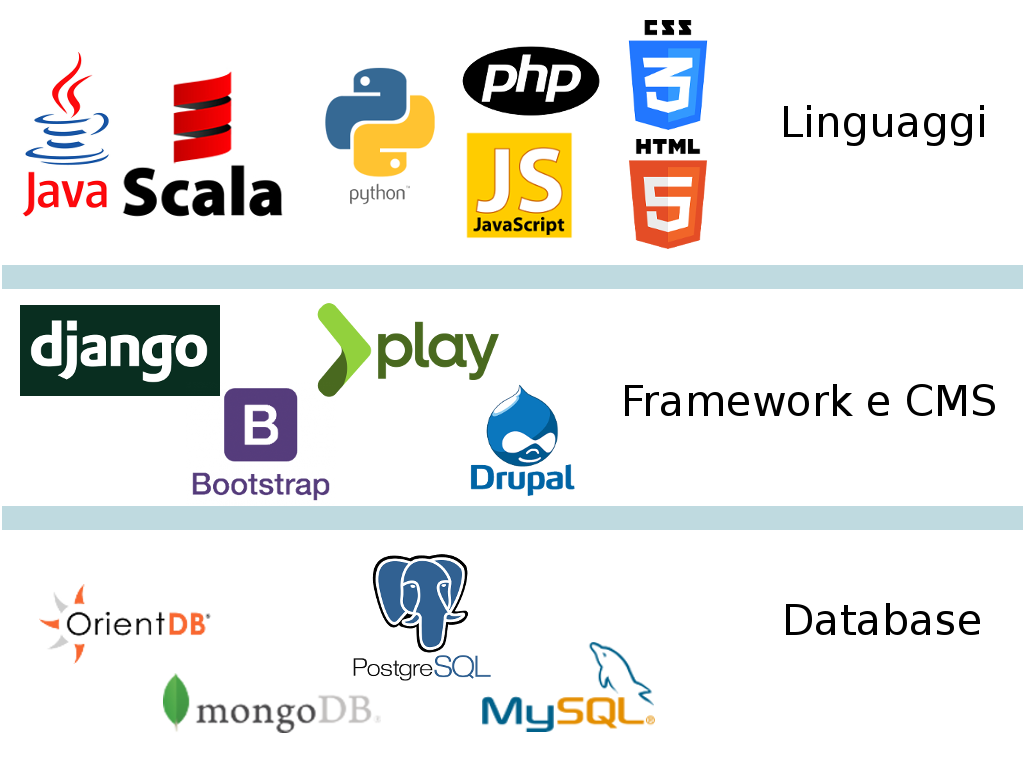
\includegraphics[scale=0.35]{immagini/tecnologie}
\caption{Classificazione delle tecnologie utilizzate}
\label{fig:tecnologie-utilizzate}
\end{figure}

\subsubsection{Linguaggi di programmazione}
L'azienda lavora principalmente in ambito \emph{web}, quindi utilizza i linguaggi di programmazione più moderni per lo sviluppo dei prodotti. I linguaggi di programmazione più utilizzati in ordine di importanza sono: Php, Python, Java e Scala. Per quanto riguarda le interfacce grafiche naturalmente utilizza tecnologie quali Html5, Css3 e Javascript.

\subsubsection{Framework e CMS}
\begin{description}
\item[Django] è un \emph{web \gls{framework} open source} per lo sviluppo di applicazioni \emph{web}, scritto in linguaggio Python, seguendo il \emph{pattern} \gls{mvc}. Fornisce nativamente delle applicazioni, per la gestione dei contenuti e degli accessi.
\item[Play Framework] è un \emph{web \gls{framework} open source} scritto in Java e Scala, che implementa il \emph{pattern} \gls{mvc}. Il suo scopo è di migliorare la produttività degli sviluppatori, usando il paradigma \emph{Convention Over Configuration}.\newpage
\item[Bootstrap] è \gls{framework} per la creazione di siti e applicazioni per il \emph{web}. Essa contiene modelli di progettazione basati su Html e Css. Necessarie per la tipografia, che per le varie componenti dell'interfaccia come moduli, bottoni e navigazione, e altri componenti dell'interfaccia.
\item[Drupal] è una piattaforma \emph{software} di \emph{\gls{cms}}, modulare, scritta in linguaggio Php e distribuita sotto licenza GNU GPL. Grazie alla sua architettura modulare, permette il riutilizzo sistematico del codice scritto e quindi un vantaggio, in termini di tempo e manutenzione.
\end{description}

\subsubsection{Database}
Il \emph{team} di sviluppo utilizza per la persistenza sia \emph{database} relazionali, sia non-relazionali.\\Fra i \emph{database} relazionali impiega per la maggiore le tecnologie quali MySql, Sql Server e PostgreSql. Per quanto riguarda i \emph{database} non-relazionali utilizza soluzioni come MongoDB oppure OrientDB. A seconda del contesto vengono studiati i pro e contro, in modo da poter trarre tutti i vantaggi possibili.
%***************************************************************************************




%***************************************************************************************
\newpage
\section{Processi aziendali}
Questa sezione illustra l'organizzazione interna dell'azienda, descritta per processi.
\begin{figure}[h]
\centering
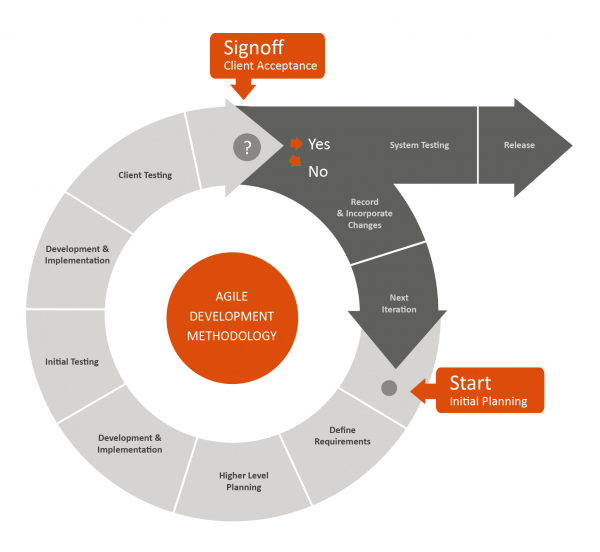
\includegraphics[scale=0.65]{immagini/agileo}
\caption{Diagramma della metodologia di sviluppo \emph{agile}. Immagine tratta da \href{http://blogs.globalteckz.com/characteristics-of-agile-methodology-in-software-development/}{GlobalTeckz}.}
\label{fig:agile}
\end{figure}
\subsection{Metodologia agile}
L'azienda per la gestione dei progetti adotta la metodologia \emph{agile}\footnote{\url{http://www.agilemanifesto.org/}}.\\Questa metodologia si basa su 4 principi:
\begin{itemize}
\item Gli individui e le interazioni più che i processi e gli strumenti;
\item Il \emph{software} funzionante più che la documentazione esaustiva;
\item La collaborazione col cliente più che la negoziazione dei contratti;
\item Rispondere al cambiamento più che seguire un piano.
\end{itemize}
In particolare tra le metodologie \emph{agile} l'azienda segue nello specifico il modello \emph{Scrum}, dove pianifica ciclicamente degli \emph{sprint}(un periodo di 2-4 settimane).
\newpage
Gli elementi costruttivi principali in \emph{Scrum} sono:
\begin{itemize}
\item \textbf{Product Backlog}, è un documento ad alto livello per l'intero progetto. Contiene una lista delle funzionalità desiderate, con priorità assegnate in base al valore di \emph{business} e  i \emph{Backlog Item} che sono descrizioni di tutte le caratteristiche richieste;
\item \textbf{Sprint Backlog}, è un documento che contiene informazioni su come il \emph{team} sta procedendo nell'implementare le funzionalità, per lo \emph{sprint} successivo. Le funzionalità vengono prelevate dalla pila del documento di \emph{Product Backlog}, in una quantità fattibile per essere realizzata nello \emph{sprint};
\item \textbf{Burn Down Chart}, è un grafico che rappresenta il lavoro nello \emph{Sprint Backlog} che deve essere ancora completato. Aggiornato ogni giorno, dà una semplice visione di come procede lo \emph{sprint};
\item \textbf{Incremento}, è la somma di tutti gli elementi del \emph{Product Backlog}, completati durante uno \emph{sprint} e tutti gli \emph{sprint} precedenti.
\end{itemize}
Le principali pratiche che Nextep svolge sono:
\begin{itemize}
\item \textbf{Daily scrum}, detto anche \emph{stand up}, è una riunione che tiene quotidianamente e serve per verificare lo stato di avanzamento durante uno \emph{sprint};
\item \textbf{Scrum of Scrums}, è una riunione che tiene meno frequentemente del \emph{Daily Scrum}. Consente ai \emph{team} di discutere del loro lavoro, concentrandosi su aree di sovrapposizione e d'integrazione;
\item \textbf{Sprint Planning Meeting}, è una riunione che l'azienda svolge all'inizio di ogni \emph{sprint}. Vengono pianificati gli obiettivi con relative priorità e le tempistiche. In questa riunione, partecipano \emph{Product Owner}, \emph{Scrum Master}, intero \emph{Scrum Team} e tutti i \emph{manager} del caso interessati o dai rappresentanti della clientela;
\item \textbf{Sprint Review}, al termine dello \emph{sprint} l'azienda svolge questa riunione per ispezionare l'incremento e adattare, se necessario, il \emph{Product Backlog}. In conformità a questo e dei cambiamenti al \emph{Product Backlog}, fatti durante lo \emph{sprint}, i partecipanti pianificano il prossimo incremento;
\item \textbf{Sprint Retrospective Meeting}, si svolge dopo la \emph{Sprint Review}, in questa occasione lo \emph{Scrum Team} ispeziona se stesso e crea un piano di miglioramento, da attuare durante il successivo \emph{sprint}.
\end{itemize}
\begin{figure}[h]
\centering
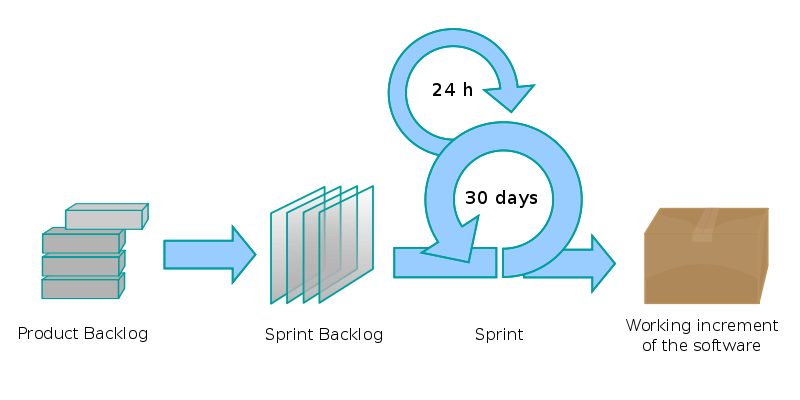
\includegraphics[scale=0.35]{immagini/scrum}
\caption{Diagramma del modello \emph{Scrum}. Immagine tratta da \href{https://it.wikipedia.org/wiki/Scrum_(informatica)}{Wikipedia}.}
\label{fig:scrum}
\end{figure}
\newpage
Questa metodologia consente e promuove un maggiore coinvolgimento del cliente rispetto a quelle tradizionali. Consente inoltre una maggiore flessibilità e reattività al cambio dei requisiti che possono avvenire in corso d'opera.
%***************************************************************************************




%***************************************************************************************
\section{Strumenti a supporto dei processi}
Questa sezione, illustra gli strumenti utilizzati a supporto dei processi e le tecnologie utilizzate per lo sviluppo.
\subsection{Gestione di progetto}
Per fornire assistenza ai clienti l'azienda utilizza Zendesk\footnote{\url{https://www.zendesk.it/}}, che è uno strumento che permette di centralizzare tutti i canali di comunicazione tra i quali \emph{social network}, \emph{email} e telefono. Inoltre fornisce una panoramica generale, della prestazione dell'assistenza e della soddisfazione del cliente.\\Per la gestione di progetto invece utilizza lo strumento Jira\footnote{\url{https://www.atlassian.com/software/jira}}, che fornisce degli strumenti per la gestione di sviluppo agile con il modello \emph{Scrum}, utilizzato nell'azienda. Nello specifico, Jira permette:
\begin{itemize}
\item Assegnazione dei \emph{ticket} tra i membri del \emph{team} di sviluppo;
\item Segnalazione di \emph{issue};
\item Integrazione con il sistema di \emph{repository};
\item Pianificazione dello \emph{sprint}.
\end{itemize}
\begin{figure}[h]
\centering
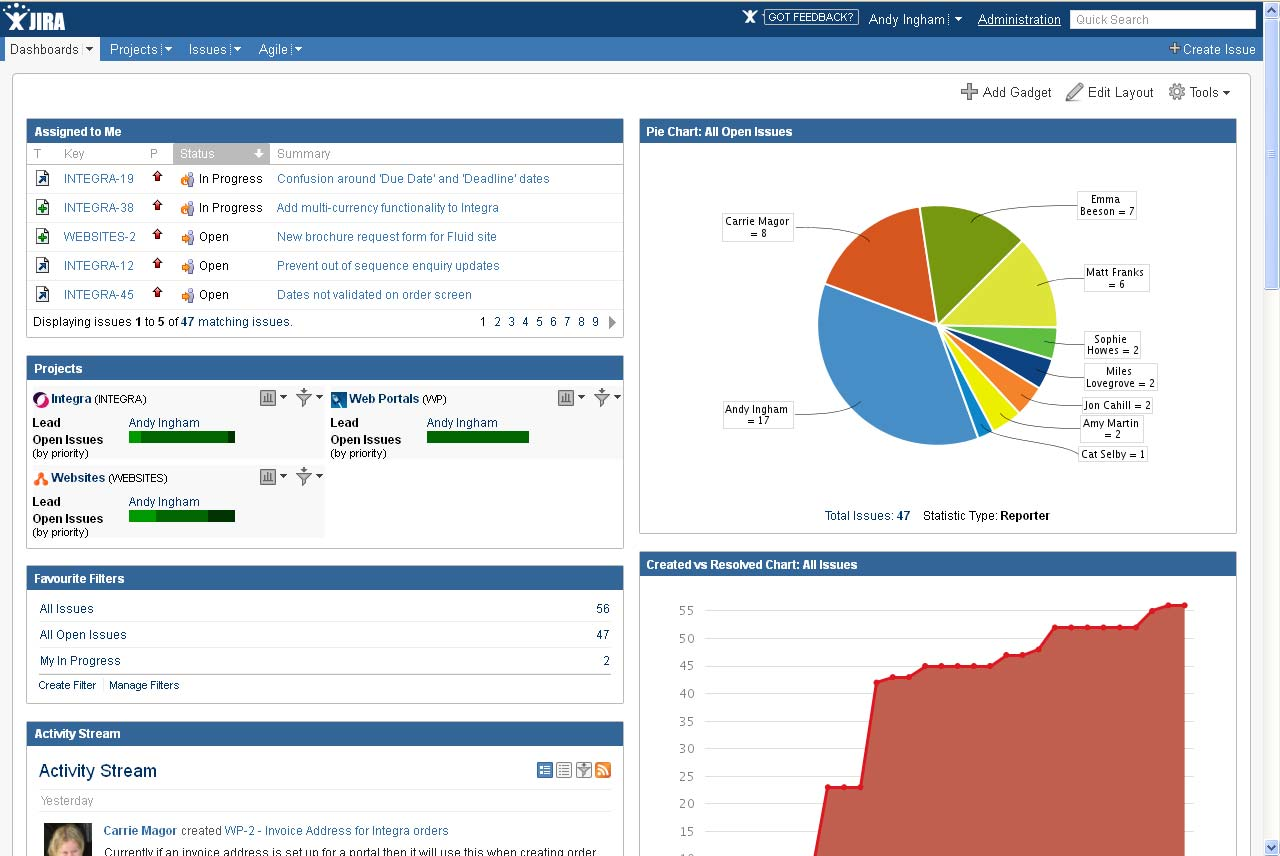
\includegraphics[scale=0.4]{immagini/jira}
\caption{Piattaforma di gestione di progetto Jira}
\label{fig:jira}
\end{figure}
Nextep non utilizza la \emph{Kanban Board} integrata in Jira, perché questo strumento di processo non è compatibile con la metodologia \emph{agile} in uso. Pertanto adopera una \emph{Scrum Board} fisica presente in ufficio.
\newpage
\subsection{Documentazione}
Nextep per la produzione documentale utilizza una serie di strumenti di Google Docs, per una serie di fattori tra i quali:
\begin{itemize}
\item Compatibilità con tutti i sistemi operativi utilizzati;
\item Permette di lavorare collaborativamente ai documenti;
\item Disponibilità;
\item Affidabilità.
\end{itemize}
\subsection{Sistema di versionamento}
Come sistema di versionamento, il \emph{team} utilizza lo strumento di Git\footnote{\url{https://git-scm.com/}}.\\I \emph{repository} sono gestiti in un \emph{server} locale, ed occasionalmente in server esterni.
\subsection{Ambiente di sviluppo}
A seconda del contesto, il \emph{team} utilizza l'ambiente di sviluppo che meglio si adatta alle tecnologie in uso nel progetto. In particolar modo adopera i seguenti \gls{ide}:
\begin{itemize}
\item Eclipse o IntelliJ: per lo sviluppo di applicazioni in Java e/o Scala;
\item Smultron/PhpStorm: per lo sviluppo di applicazioni in Php;
\item Sublime Text: per lo sviluppo in Html/Css, Javascript e Php.
\end{itemize}
\newpage
\subsection{Sistemi operativi}
L'azienda non impone nessun obbligo di utilizzo di un sistema operativo.\\I dipendenti utilizzano, a seconda delle preferenze, sistemi operativi quali Windows, Linux e MacOs. In particolar modo quest'ultimo, visto il recente investimento aziendale in nuovi terminali. Il fine è di incentivare i dipendenti, alla migrazione a questo sistema operativo.
\begin{figure}[h]
\centering
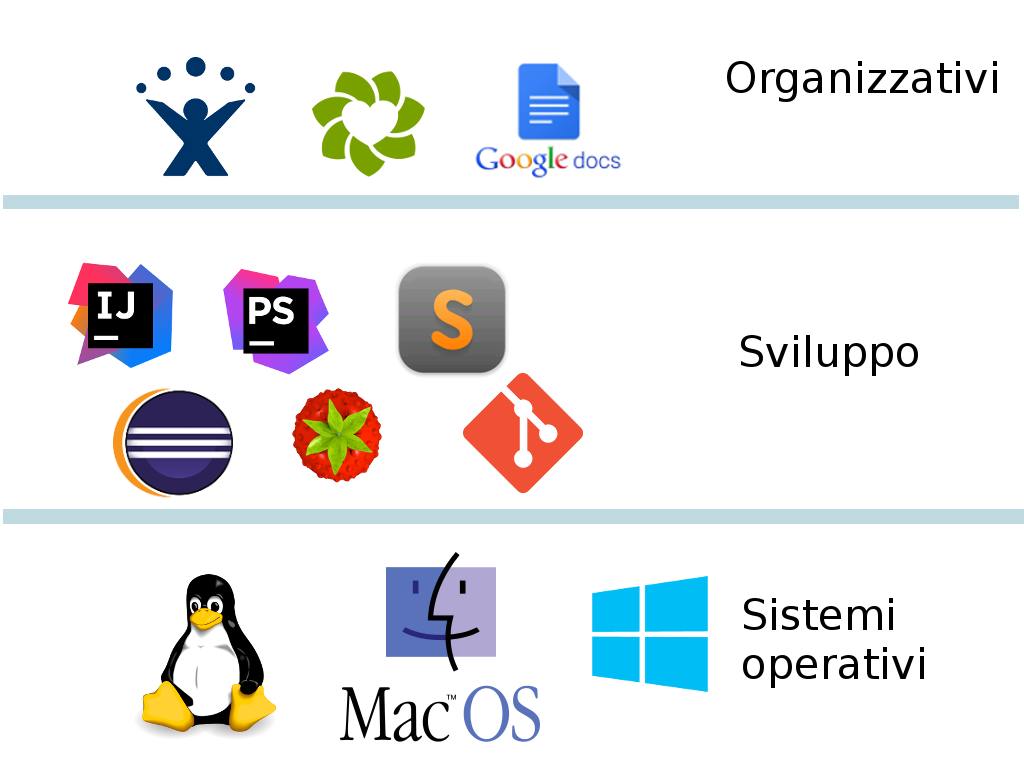
\includegraphics[scale=0.25]{immagini/strumenti}
\caption{Classificazione degli strumenti utilizzati}
\label{fig:strumenti}
\end{figure}
%********************************************************************************************




%********************************************************************************************
\section{Clientela tipo e propensione all’innovazione}
La tipologia di clientela per cui l'azienda lavora, copre una gamma che va dal singolo privato alle organizzazioni di grandi dimensioni.\\Essendo gli \emph{e-commerce} il \emph{core business} dell'azienda, Nextep lavora principalmente per aziende dell'ambito manifatturiero e rivendite.\\L'azienda lavora per clienti/aziende italiane e molto spesso per clienti della zona, visto il riconoscimento guadagnato nel padovano.\\Nextep riconosce questi valori guida da seguire:
\begin{itemize}
\item Attitudine all'innovazione per mantenere competitività;
\item Condivisione del \emph{know how} con le altre aziende in sede.
\end{itemize}
Questi principi rendono possibile un ambiente di \emph{co-working}, dove le 3 aziende della sede sperimentano e innovano, grazie alle conoscenze messe in condivisone. Per alimentare questa dinamica, l'azienda promuove periodicamente la formazione dei dipendenti, in modo che essi possano essere motivati e partecipi in questo ambiente. Visto l'importanza delle dinamiche personali, l'azienda organizza, al bisogno, degli incontri di \emph{team building} per avere sempre dei dipendenti in grado di lavorare in gruppo.  
%**************************************************************
